\documentclass[11pt, a4paper, landscape]{article}
\usepackage[english,userlastpage,triangle,utf-8]{NeyDreuwSlides_Oct08}
\usepackage{algorithm}
\usepackage{algpseudocode}
\usepackage{tikz}
\usepackage{pifont}
\usepackage{wasysym}
\usepackage{amssymb}
\usepackage{pdfpages}
\usepackage{color}

\renewcommand*{\title}{ASR Lab Results}                               % main title of the work (used for \TitlePage)
\renewcommand*{\titleshort}{ASR Lab Results}                    % short title (used for \lfoot)
\renewcommand*{\occasion}{Presentation} % (used for \TitlePage)
\renewcommand*{\occasionshort}{~}  % short occasion title (used for \rfoot)
\renewcommand*{\date}{\today}
\renewcommand*{\author}{Ilya Sklyar, Konstantin Kromberg, Miguel Gra\c{c}a}                                     % all the authors of the work, can be long (used for \TitlePage)
\renewcommand*{\authorshort}{Sklyar, Kromberg, Gra\c{c}a~~}                                        % all the authors of the work, should be short (used for \lfoot)
\renewcommand*{\email}{~}             % all email address(es) of the authors (used for \TitlePage)
\renewcommand*{\mainauthor}{Ilya Sklyar, Konstantin Kromberg, Miguel Gra\c{c}a}                                 % the author(s) who presented the work (used for \FinalPage)
\renewcommand*{\mainauthoremail}{\email}                                  % presenter mail address(es) (used for \FinalPage)
\renewcommand*{\www}{~}            % web address (used for \TitlePage _and_ \FinalPage)
\newcommand*{\keywords}{Title of Presentation, etc.}      % keywords for pdf summary
\renewcommand{\arraystretch}{1.2}

% will be set into the PDF document summary
\hypersetup{
  pdftitle={\title}, 
  pdfsubject={\occasion},  
  pdfauthor={\author}, 
  pdfkeywords={\keywords}
}

%%%%%%%%%%%%%%%%%%%%%%%%%%%%%%%%%%%%%%%%%%%%%%%%%%%%%%%%%%%%%%%%%%%%%%%%%%%%%%%%
\usepackage[insection]{minitoc}
\renewcommand{\stifont}{\normalsize\bf} 
\renewcommand{\stcfont}{\normalsize\bf}
\renewcommand{\stcSSfont}{\normalsize\bf}

\begin{document}

%%%%%%%%%%%%%%%%%%%%%%%%%%%%%%%%%%%%%%%%%%%%%%%%%
\TitlePage

%%%%%%%%%%%%%%%%%%%%%%%%%%%%%%%%%%%%%%%%%%%%%%%%%
\NewPage\headline{Overview}
\vfill
\begin{itemize}
  \item Testing Environment
  \item Gaussian Mixture Model (GMM) Tuning
  \begin{itemize}
    \item Expectation-Maximization (EM) Parameters
    \item Alignment Parameters
    \item Search Results
  \end{itemize}
  \item Neural Network (NN) Tuning
  \begin{itemize}
    \item Write stuff here
    \item Search Results
  \end{itemize}
\end{itemize}
\vfill

%%%%%%%%%%%%%%%%%%%%%%%%%%%%%%%%%%%%%%%%%%%%%%%%%
\NewPage\headline{Testing Environment}
\vfill
Hardware:
\begin{itemize}
  \item Intel i5-4690K @ 3.5GHz, Quad Core, SSE2 registers
  \item 16GB DDR3 1333MHz RAM
\end{itemize}
\vspace{20pt}
Parallelization with OpenMP:
\begin{itemize}
  \item In search
  \item In neural network operations
\end{itemize} 
\vfill

%%%%%%%%%%%%%%%%%%%%%%%%%%%%%%%%%%%%%%%%%%%%%%%%%
\NewPage\headline{GMM Tuning: EM Parameters}
\vfill
Basic setup:
\begin{itemize}
  \item Lexicon consists of 106 states
  \item Exact computation of the linear segmentation
  \item 6 EM steps
  \item 4 density splits
\end{itemize} 
\vspace{20pt}
Tunable properties:
\begin{itemize}
  \item Minimum observations per density
  \item Pooling type
\end{itemize}
\vspace{20pt}
Tuning is based on the likelihood of the training data
\vfill

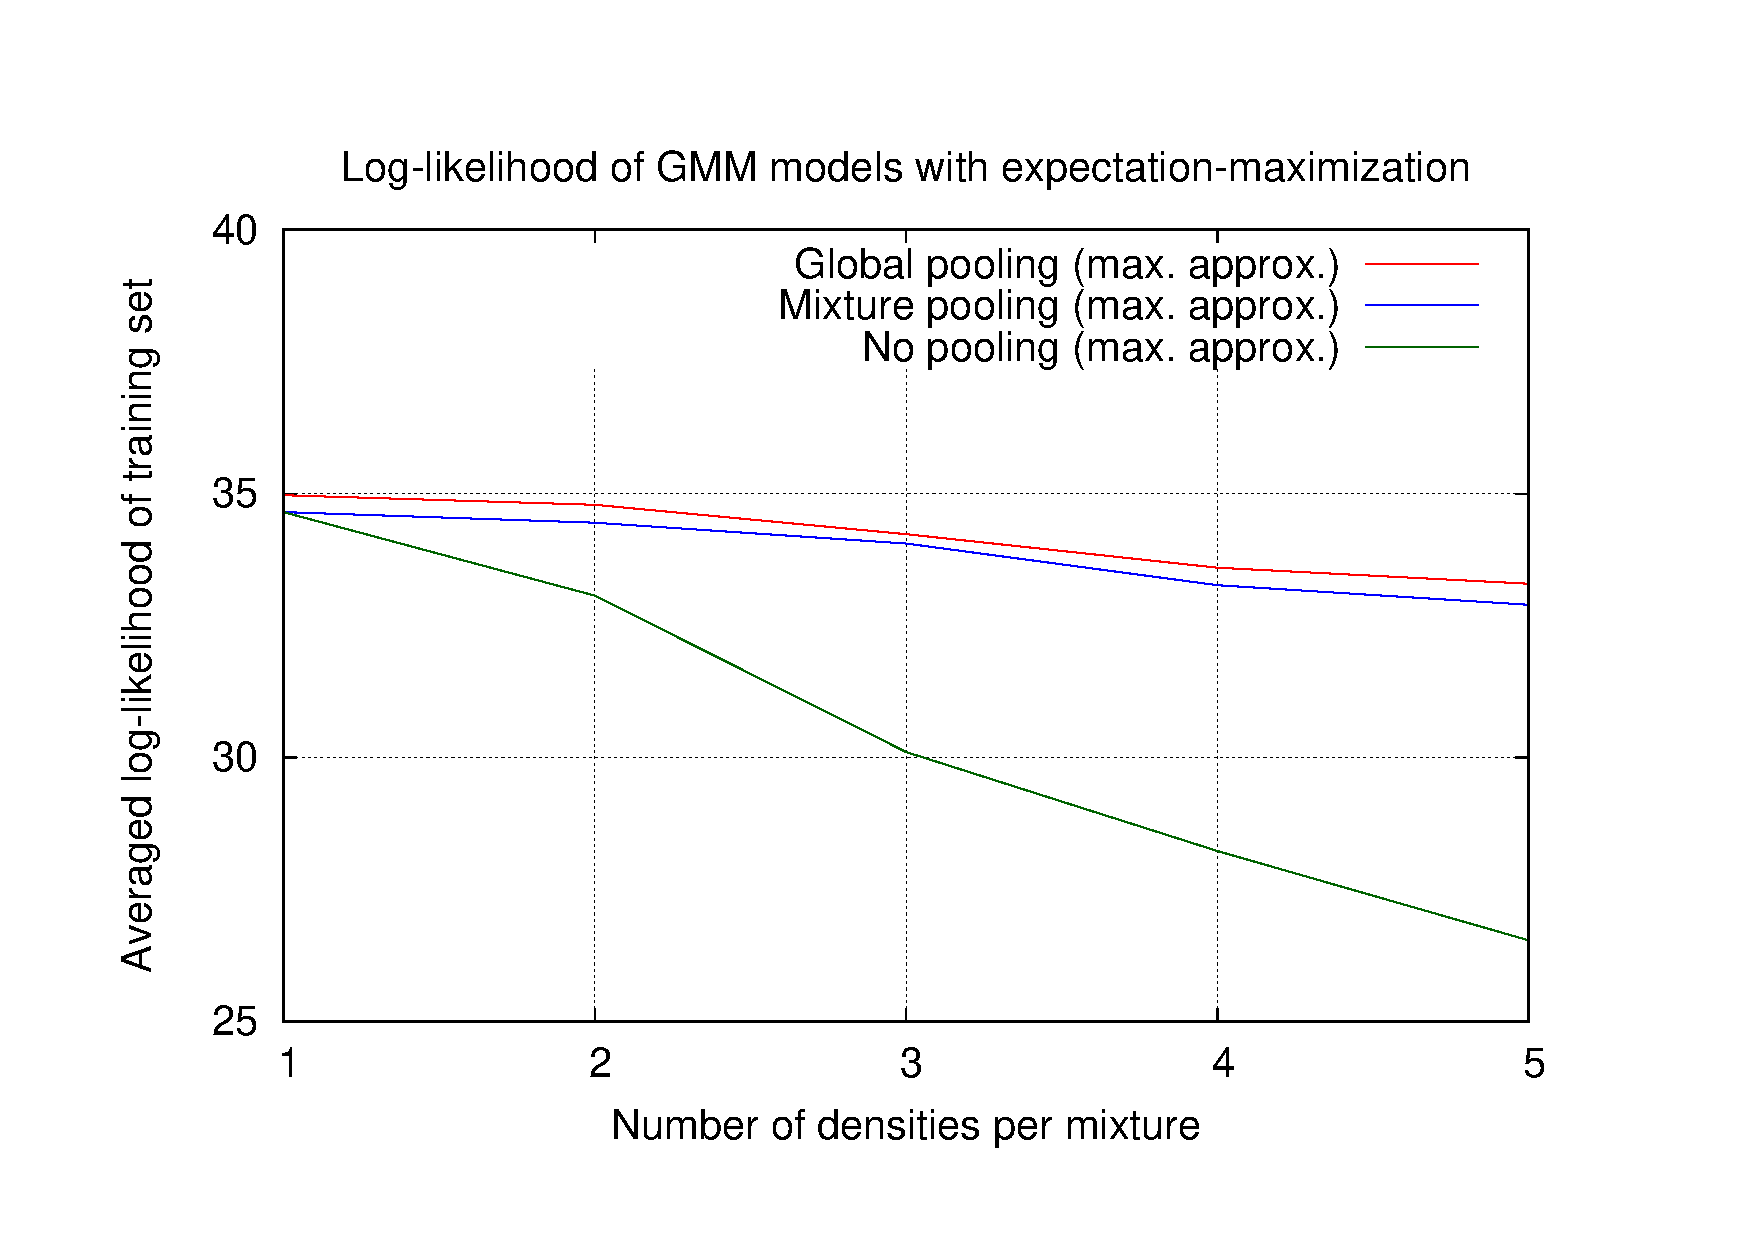
\includepdf[pages=-]{plots/am_score_afterSplit.pdf} 

%%%%%%%%%%%%%%%%%%%%%%%%%%%%%%%%%%%%%%%%%%%%%%%%%%%
\NewPage\headline{GMM Tuning: EM Parameters}
\vfill
Pooling:
\begin{itemize}
	\item No pooling results in better model fitting than using pooling 
	\item Global and mixture-level pooling perform similarly 
  \item Due to the size of the data, there is little reason to use pooling
\end{itemize}
\vspace{20pt}
Splitting criterion:
\begin{itemize}
	\item Minimum number of observations per density has a small influence
	\item Sufficient data points per density in a mixture due to:
	\begin{itemize}
		\item At most $5$ densities per mixture
		\item Each density has, in average, $7$K data points.
	\end{itemize}
\end{itemize}
\vfill

%%%%%%%%%%%%%%%%%%%%%%%%%%%%%%%%%%%%%%%%%%%%%%%%
\NewPage\headline{GMM Tuning: Alignment Parameters}
\vfill
Tunable parameters (optimized on the best performing EM setup):
\begin{itemize}
	\item Time distortion penalty (TDP) values:
    \begin{itemize}
      \item Forward transitions do not have costs (to enforce monotonicity)
      \item Skip and loop transitions have differing costs
    \end{itemize}
	\item Pruning threshold: 50-1000 (still have to do)
\end{itemize}
Optimized parameter values:
\begin{itemize}
	\item TDP : 3-0-30
	\item Word penalty: 80
	\item AM threshold: 200\\
\end{itemize}
\vfill

%%%%%%%%%%%%%%%%%%%%%%%%%%%%%%%%%%%%%%%%%%%%%%%%
\NewPage\headline{Alignment Results}
\vfill
\begin{itemize}
  \item Evaluation on acoustic model (AM) score and silence ratio in resulting alignment
  \item Pruning threshold set to 200
  \item TDP format (Skip-Forward-Loop) 
\end{itemize}

\begin{center}
\begin{tabular}{| l |  c | c |} \toprule
  TDP values & AM score     & Silence [\%] \\ \midrule
  1-0-10     & yolo         & yolo         \\
  2-0-20     & yolo         & yolo         \\
  3-0-30     & \alert{yolo} & \alert{yolo} \\ \midrule
  10-0-10    & yolo         & yolo         \\
  20-0-20    & yolo         & yolo         \\
  30-0-30    & yolo         & yolo         \\ \bottomrule
\end{tabular}
\end{center}
\vfill


%%%%%%%%%%%%%%%%%%%%%%%%%%%%%%%%%%%%%%%%%%%%%%%%
\NewPage\headline{Search Results}
\vfill
Final results with optimized parameters on test corpus:
Word penalty: 60-120
\begin{itemize}
	\item[=>] WER: 4.703562\%
	\item[=>] SER: 12.335138\%
	\item[=>] RFT: 0.437114
\end{itemize}
\vfill

%%%%%%%%%%%%%%%%%%%%%%%%%%%%%%%%%%%%%%%%%%%%%%%%
\NewPage\headline{Last week}
\vfill
\vfill

%%%%%%%%%%%%%%%%%%%%%%%%%%%%%%%%%%%%%%%%%%%%%%%%
\NewPage\headline{Last week}
\vfill
\vfill

%%%%%%%%%%%%%%%%%%%%%%%%%%%%%%%%%%%%%%%%%%%%%%%%
\NewPage\headline{Last week}
\vfill
\vfill
\FinalPage
\end{document}
